\documentclass[11pt,a4paper]{report}

\usepackage[a4paper,
			twoside,
			left=1.5in,
			right=1.0in,
			height=9.0in,
			headheight=14pt]{geometry}
\usepackage{fancyhdr}
\pagestyle{fancy}
\cfoot{}
\fancyhead[LE,RO]{\thepage}

\usepackage{url}
\usepackage[utf8x]{inputenc}
\usepackage{ucs}
\usepackage{amsmath}
\usepackage{amsfonts}
\usepackage{amssymb}
\usepackage{graphicx}
\usepackage{natbib}
\usepackage{multicol}
\usepackage{subcaption}
\usepackage{makecell}
\usepackage[hidelinks]{hyperref}
\usepackage{rotating}
\usepackage[toc,page]{appendix}
\usepackage{epstopdf}


% Code snippet setup ---- START
\usepackage{listings}
\renewcommand{\lstlistingname}{Snippet}
\usepackage{color}
\definecolor{dkgreen}{rgb}{0,0.6,0}
\definecolor{gray}{rgb}{0.5,0.5,0.5}
\definecolor{mauve}{rgb}{0.58,0,0.82}
\lstset{frame=tb,
  language=Matlab,
  aboveskip=3mm,
  belowskip=3mm,
  showstringspaces=false,
  columns=flexible,
  basicstyle={\small\ttfamily},
  captionpos=b,
  numbers=left,
  numbersep=5pt,
  stepnumber=5,
  firstnumber=1,
  numberstyle=\tiny\color{gray},
  keywordstyle=\color{blue},
  commentstyle=\color{dkgreen},
  stringstyle=\color{mauve},
  breaklines=true,
  breakatwhitespace=false,
  tabsize=3
}
% Code snippet setup ---- END

\author{
	Christensen, Daniel\\
	\texttt{\href{mailto:dhch12@student.aau.dk}{dhch12@student.aau.dk}}
	\and
	Høeg, Emil Rose \\
	\texttt{\href{mailto:ehaeg12@student.aau.dk}{ehaeg12@student.aau.dk}}
	\and
	Lind, Rasmus Bloustrød\\
	\texttt{\href{mailto:rlind12@student.aau.dk}{rlind12@student.aau.dk}}
	\and
	Nilsson, Sam Alix \\
	\texttt{\href{mailto:snilss12@student.aau.dk}{snilss12@student.aau.dk}}
	\and
	Smed, Dina Madsen\\
	\texttt{\href{mailto:dsmed12@student.aau.dk}{dsmed12@student.aau.dk}}
	\and
	Sørensen, Casper\\
	\texttt{\href{mailto:csare12@student.aau.dk}{csare12@student.aau.dk}}
	\and
	Vinkel, Simone Patricia \\
	\texttt{\href{mailto:svinkel12@student.aau.dk}{svinkel12@student.aau.dk}}
}
\title{{\LARGE \textbf{Automatic Transcription of Beatboxing}} \\
{{\Large By group 403}}}


% BACKGROUND ---- START
\usepackage{eso-pic}
\newcommand\BackgroundPic{%
\put(0,0){%
\parbox[b][\paperheight]{\paperwidth}{%
\vfill
\centering
\includegraphics[width=\paperwidth,height=\paperheight,%
keepaspectratio]{fig/Background.png}%
\vfill
}}}
% BACKGROUND ---- END

\begin{document}
% Add background
\AddToShipoutPicture*{\BackgroundPic}
% when i (Rasmus B. Lind) quick build the pdf the next line makes trouble  

\maketitle
\tableofcontents
\chapter{Introduction}
\thispagestyle{empty}
\section{ Introduction }
\subsection{ Imitation of Instruments }
Let’s not mention the old greeks, german yodeling, or the lullabies of our mothers, but instead start from the modern utilization of musical instruments and rhythmic compositions. In the modern ages people have had the need to imitate instruments for several reasons. One is to describe melodies, rhytms, tones and feelings in the creation of music to others. Another reason could be the lack of instruments while still wanting to socially interact with others and to perform complex instrumental patterns vocally. Lastly simply because we as human beings get songs in our heads and intuitively burst out into humming and imitating music we’ve heard because we can’t stop it. One can say that we have had the need to imitate instrumental sounds since the invention of music.
\subsection{ Vocal Percussion }
Using mouth, lips and throat to produce percussion sounds and effects is seen in many cultures all through history. North American scat singing, African Khoisan i.e. Click Language (e.g. Xhosa from South Africa and Khoekhoe from Botswana) are among the cultural examples (Choi, 2013).	
The modern day equivalent is known as Beatboxing which is primarily linked to the early hip-hop-culture in the 1980’ies. The self-proclaimed pioneer of Beatboxing, Doug E. Fresh also known as ‘The Human Beatbox’ was a key player in making Beatboxing famous. However, other earlier artists has been known to use similar techniques of vocal percussion in published material e.g. Paul McCartney with the song “That Would Be Something” from 1969.
\subsection{ Beatboxing }
Human Beatboxing is generally limited to percussive sounds produced by the vocal cord and body (e.g. clapping) to imitate rhythms of a drumset i.e. snare drum, hi-hat, kick drums, cymbals etc. but some Beatboxers also imitates bass and guitar and occasionally combined with vocal. An example of this is Michael Winslow, an American comedian, actor, and beatboxer probably best known for his ability to make realistic sound effects with his voice in the movie Police Academy (1984). Beatboxing as an artform was an outspring of the hip hop culture since the 1980’ies. It was shaped by musical technologies in context with its age, and through time it evolved to become a complex instrumental expression. In the origin of human beatboxing it was meant to imitate grooves and beats but soon it utilized sounds like basslines, scratching, effects, noise, and almost every musical instrument and “filters”. –With improved techniques and sophisticated microphone technology beatboxing became a modern instrumental element in many music genres of today.
\subsection{ Software to transcribe instruments }
Since “modern beatboxing” evolved, it seems like technology is reclaiming it’s technological importance. Some artists are beginning to transcribe instruments, adding filters and effects to beatboxing which takes the complexity of beatboxing even further. I.e. Dub FX, Benjamin Stanford from Australia, who samples sequences of vocal basslines, grooves and adds effects to them. Lately he re-recorded ‘Love Someone’ using Roland RC-505, a so called ‘Loop Station’, based on sequential recording of each track in instrumental compositions. [2] This way, he can perform on streets as one person, sounding as an orchestra. ** NEED TO WRITE MORE ON TRANSCRiPTION**
\\
\begin{figure}[h]
	\begin{center}
		\includegraphics[height=5cm]{fig/Roland-RC-505.JPG}
		\caption{Roland Looper RC-505}
		\label{Looper}
	\end{center}
\end{figure}
\\
\subsection{ Motivation }
The motivation of this project is the admiration of innovative artforms and to explore the opportunities that arise from them. It is the fact that any analog instrument can be treated as a source for digital and electronic processing. Paradoxically beatboxing comes from imitating other analog instruments, but every other analog instrument is also victimized by digitalization. Jimi Hendrix pushed the creative scope of playing guitar, Jean Michel Jarre by playing piano and electronic drums. Why shouldn’t beatboxing be treated as an analog instrument as well? 
\subsection{ Why Beatboxing? }
The good thing about beatboxing is that it is under constant adaption to modern instrument technologies. It’s intuitively the fast way forward to learn grooves and rhythms. Beatboxing comes easy to many even though it requires one to let go of shyness, -like any other instrument. The good thing about beatboxing is that it comes relatively easy to many people. It only requires creativity to imitate sounds and instruments, while many people also tends to have the ability of humming with decent outcome. If technology can provide additional possibilities to facilitate the creation music that sounds good, it can be a fun way to learn the principles of rhythm and to produce satisfactory music, even that one does not know the basics or the techniques of a traditional instrument. 

\chapter{Background}
\thispagestyle{empty}

\section{Beatboxing as an Artform}
Beatboxing as an artform originated from the hip hop culture back in the 1980s  \citep{Stowell2010}. It was derived by vocally imitating drum-machines known as beatboxes e.g. the Roland TR808, which was often used in the production of hip hop music, as a way to create grooves and beats using the mouth, nose and throat \citep{proctor2012}. The self-proclaimed pioneer of beatboxing, Doug E. Fresh also known as the "The Original Human Beatbox", was a key player in promoting beatboxing as an artform. Other mentionable artists were Darren Robinson (Fat Boys), Biz Markie and Rahzel, who also shaped and improved the techniques used in beatboxing \citep{Hess2007}.

While beatboxing primarily involves the imitation of percussive sounds, other beatboxers attempts to imitate bass, guitar or other effects. An example of this is Michael Winslow, an American comedian, actor and beatboxer, probably best known for his ability to make sound effects e.g. imitation of phones or helicopters with his voice in the movie \textit{Police Academy} from 1984. 

Through time beatboxing has evolved to become a complex instrumental expression and an artform which is constantly advancing and adapting to modern instruments and audio technologies \citep{proctor2012}. Take for example the beatboxer Tom Thum who authentically imitates the pounding techno-rhythm from within a night club at a TEDx conference \citep{TEDx}. With improved techniques and sophisticated microphone technology beatboxing has become an instrumental element in many music genres besides hip hop, and has as an example been used in pop-music by The King of Pop Michael Jackson\footnote{\url{https://www.youtube.com/watch?v=LQuKbzWHvIo}}.

On an international scale the internet has contributed to the growing popularity of beatboxing, especially with the establishment of the Human Beat Box-community by Alex Tew, who subsequently created the first ever beatboxing convention\footnote{\url{www.beatboxconvention.com}} in 2003; a convention which succeeded in assembling beatboxers from all over the world\footnote{\url{www.humanbeatbox.com}}.
The community is also behind the first beatboxing tutorials that were published in 2003. Furthermore Gavin Tyte and Mark Splinter developed the Standard Beatbox Notation (SBN) as a simple and consistent method to describe sounds and rhythms used in human beatboxing \citep{Tyte}.
\section{Other vocal music practices}

Besides hiphop, vocal percussion techniques are seen in many cultures \citep{Sinyor05}. E.g. “scat singing”, mainly seen in jazz, by applying rhythmic nonsense syllables to singing, also referred to as "onomatopeia". I.e. by Ella Fitzgerald and Louis Armstrong \citep{Janer_syllablingon}. Vocal percussion is also seen in many other contexts, both practically, artistically and pedagogical as described briefly in this chapter.
\subsection{ Artistic Purposes}
Vocal imitation of percussion also comes in humorous variations as in the southern American predecessor to beatboxing called "Eefing", described as "a kind of hiccupping, rhythmic wheeze". Known artists as Joe Perkins hit the charts in 1963 with the song "Little Eeefin' Annie" featuring Jimmie Riddle, who was acknowledged for his skills in the genre at the time \citep{jennifersharpe2006}. In northern India recitation of solkattu \footnote{\url{ www.youtube.com/watch?v=d1yN96ZDGm8}} known as “Konnakol” \citep{proctor2012}. Celtic lilting and diddling \footnote{\url{www.youtube.com/watch?v=Rm_oaqW_qRM&list=PLUgNSFkRKerlocdy-qiC2Z879JlH-FfHe}} also have the characteristics of percussive elements \citep{proctor2012}.
\subsection{ Pedagogic Purposes}
Vocal emulation has also been employed to imitate instruments for pedagogic purposes. For example to teach Cuban percussion, "Vayttari" Indian music, Peking opera and Japanese Noh flute \citep{Janer_syllablingon}. For drum notations “changgo” is used in Korea, as vocables for samul nori drumming, whereas Cuban conga players vocalize motifs as “guauganco or tumbao patterns” \citep{proctor2012}.
\subsection{ Compositional Roles }
There are many examples of vocal emulation of instruments as some of them are mentioned above. Beatboxing, which origins from imitation of drum machines e.g. the Roland TR-808 \citep{proctor2012}, imitates the drum track and is therefore adaptable to many types of compositions. Both as a solo element and as an accompanying instrumental element. Compared to other vocal artforms, in particular the artforms mentioned in this chapter, beatboxing can be said to be the most dynamic and evolving form of vocal percussion as it is based on imitation of all modern instruments. Compared to its predecessor “eefing”, beatboxing is less dominating in the rhythmic composition, where many of the other mentioned vocal artforms are also relatively dominant, and are preferably used as solo elements in compositions. Lastly, beatboxing is a relatively new performance style \citep{Stowell2008}, but it is still widely embraced in mainstream music as in the underground hiphop environment. Beatboxing imitates both humorous elements and pure a capella expressions, which makes it interesting to utilize in many contexts. 
As it is widely utilized in the mainstream music industry, and known by some generations in modern ages, it becomes interesting to develop even further or reinvent certain technical aspects for the performing artists and providers of music technology. Which can also be said to be the background and motivation of the further studies.

\chapter{Methods of Beatboxing-transcription}
\thispagestyle{empty}
\section{intro}
This section will contain what works that are similar to the proposed problem of beatbox transcription, first of some application that uses beatboxing or methods like beatboxing will be presented. Then some article that was found during research will be presented and the main point will be described. lastly some features that have been presented in the article will be described.
\section{ State-of-the-Art }
To comprehend the method of transcription, it is relevant to investigate software solutions and theoretical solutions that are approximate to the presented problem of this project. In this section the acquired applications and solutions will be presented in conjunction with the presumed relevance which is necessary to solve the problem.

\subsection{ Voice Drummer }
Voice Drummer is defined as a "percussion instrument notation interface"  \citep{VoiceDrummer}. It is a software-application developed to aid those without substantial musical knowledge to notate music. The program is limited to transcribing bass drum and snare drum, and these are differentiated between by their onomatopoeic expressions and the rhythm-pattern timing.
\\
\begin{figure}[h]
	\begin{center}
		\includegraphics[height=5cm]{fig/VoiceDrummer.png}
		\caption{An example of Voice Drummer's practice adaption-mode \citep{VoiceDrummer}.}
		\label{VoiceDrummer}
	\end{center}
\end{figure}
\\
Onomatopoeic refers to words that phonetically imitates, or resembles the source of the described sound e.g. classifying 'meow' as a sound a cat would make \citep{VoiceDrummer}. Thus, making it easy for a layman to understand, and use Voice Drummer by uttering \textit{don-don} to generate a bass drum, and \textit{ta-ta} to generate a snare drum. These are transcribed into phonemic representations through a pronunciation dictionary which will recognize and output the correct corresponding output in real-time \citep{VoiceDrummer}.

\subsection{ Voice Band }
\begin{figure}[h]
	\begin{center}
		\includegraphics[height=5cm]{fig/voiceband.png}
		\caption{A photograph of the Voice Band interface on an iPad Mini.}
		\label{VoiceBand}
	\end{center}
\end{figure}

Voice Band is an iPhone (iOS) application by WaveMachine Labs which alters your voice into sampled instruments in real-time \citep{WML2013}. It comes with a set of instruments to choose from including rhythm guitar, lead guitar, bass, saxophone, synthesizers, organ, drums and microphone, but there are other instruments and expansions available for purchase in the Voice Band store, e.g. other drum kits or strings. According to WaveMachine Labs’ website and demo videos, their target users are songwriters who want an idea or arrangement down quickly. They call it a “portable musical scratch board”. However, it might also appeal and inspire anyone else interested in music, who wants to have fun.


For every instrument, excluding the drums and cymbals, the system detects the pitch of the voice, and changes that into an instrumental output. To avoid distortion or unwanted noise, one will get the best results by using a pair of headphones, and staying in a quiet environment, because the system is very sensitive to sound. It is also recommended to use solid, pure tones with no vibrato to reach a more accurate output, and to sing with hard consonants such as ba or da, because Voice Band recognizes the start of a sound (onset detection), and it is therefore easier to detect\footnote{\url{http://www.auriaapp.com/Support/voice-band-support}}. 

As for the drums, they are divided into kick/snare (two-in-one), hi-hat and crash. The kick and snare drums are together, where quiet notes will output kick, and loud notes will output snare. However there is the possibility to adjust the sensibility on a trigger in settings, such that only kick or only snare will be outputted, not depending on the loudness of the note. This way it is possible to record kick and snare separately as well. The hi-hat system works similarly in which soft notes produces a closed hi-hat and loud notes produces an open hi-hat. Crash is for itself. For all drums, and most of the other instruments the reverberation and volume can be adjusted. 
All instruments and singing will have to be recorded separately, but on the same track. After having recorded an instrument, it will play back the previous recorded sounds while recording another one. It converts the samples into a MP3 file, which can be sent to an e-mail. 

\subsection{ Loop Station RC-505 }
\label{loopstation}
\begin{figure}[h]
	\begin{center}
		\includegraphics[height=5cm]{fig/Roland-RC-505.JPG}
		\caption{Roland Looper RC-505 \citep{ROLAND}.}
		\label{Looper}
	\end{center}
\end{figure}
The Roland Loop Station (see figure \ref{Looper}) is specifically built for beatboxers. It enables a performing beatbox artist to record and play 5 tracks simultaneously. It can also apply sound effects to the recorded tracks, which actually makes it sound closer to a synthesizer. The Loop Station can record 99 phrases, and provides 85 on-board rhythm patterns. Moreover it can be operated with hands and with foot-switches. Additionally it can be used as a MIDI controller. It has a XLR mic input, phantom power, mono/stereo instruments input, and AUX input, which makes the Roland Looper RC-505 stand out as one of the most professional build tools for beatboxers, according to Roland CONNECT, out as one of the most professional build tools for beatboxers\footnote{\url{http://www.rolandconnect.com/product_2013-04.php?p=rc-505}}.
The Loop Station is used and promoted by the Australian beatboxing-artist DUB FX\footnote{\url{http://dubfx.net/}}.
\section{Investigation}
A great amount of effort has been put into investigating possible solutions to how transcription can be achieved through sound and music computing. While many articles, books and papers on the topic has been scrutinized, three specific articles has been found to be of utmost importance to the project. The articles addresses relevant topics i.e. transcription - / and sound classification of beatboxing.

\subsection{Transcription}
In the article \textit{Towards Automatic Transcription of Expressive Oral Percussive Performances}, Amoury Hazan propose a solution to automatic transcription, that involves sound segregation, oral percussive descriptors, and machine learning techniques. Sound segregation is described as a simple method that fits well with monophonic oral percussive recordings, which requires few computing resources \citep{Hazan2005a}.	

His project aims to reduce the gap between the user and the device (keyboard, drum pad), among other things in order to offer an aid to those musicians who cannot transcript a beat they have in mind.
Through research of the taxonomy of human phonemes, and assuring perfect percussive events through segregation and transcription, the resulting drum score lack information concerning how the performer has modulated the produced sound. Thus, Hazan argues that energy and resonance frequency variation has to be defined together with effective computational methods to track them.
	
The considerations made by Hazan may serve as a benchmark tool which may suffice to serve as a possible solution to the problem. The technical description of the Tree Induction Algorithms may be an area to research, as it could serve as an inspiration regarding how to construct the software based transcription-solution.

\subsection{Sound Classification}

[INSERT ARTICLE HERE - Beatbox Classification Using ACE \textit{by} \citep{Sinyor05} ]
\\

[INSERT ARTICLE HERE - Delayed Decisionmaking in real-time Beatbox Percussion Classification \textit{by} \citep{Stowell2010} ]

\section{Features}
\subsection{Root Mean Square}
The root mean square value is as John bird tells in Engineering Mathematics \citep{Bird2007} “the square root of the mean value of the squared values of the quantity over an interval".
\\
As Bird mentions in Engineering mathematics "One of the principal applications of RMS is with alternating current and voltage". \citep{Bird2007} The alternating current (a.c.) is defined as a current which has a heating effect resembling the direct current \citep{Bird2007}.
\\
The RMS is found by doing these three steps:
(1) First take the square of the amplitude, (2) then take the mean of the squared results, (3) lastly take the square root of the results from the results of part (2)\citep{Bird2007}. Here is \cite{Bird2007} mathematical formula for RMS:

\begin{equation}\label{eq:RMS formular}
RMSy = \frac{1}{b-a}\int_a^b\mathrm{y}^{2}\,\mathrm{d}x
\end{equation}
\subsection{Zero Crossing-Zero Crossing Rate}
Zero crossing and zero crossing rate:
Zero crossing is a term normally used in image processing, electronics and mathematics. As explained by \cite{Al-Zhrani2010} in mathematics ““Zero-crossing” is a point where the sign of a function goes from negative to positive, or the other way around. This is represented by a crossing of the axis (zero value) in the graph of the function” \cite{Al-Zhrani2010}
Zero crossing is a way of measure the period of a periodic signal aka the frequency.\cite{RWW2012} \\
Usually when measure a frequency, it is smart to measure more than just one period, since by having more periods can reduce errors caused by phase noise which is caused by making perturbations (small pairs of zero crossing in regions of low energies \cite{Mallat1988} ) in zero crossings small in comparison to the period. \cite{RWW2012} \\
There is also something called zero crossing rate. ZCR according to D.S.Shete et. al is defined as the amount of times the audio waveform the crosses the zero axis.\\
\begin{equation}\label{eq:ZCR}
\upsilon_{ZC}(n)= \frac{1}{2 \kappa}\sum_{i=i_s(n)}^{i_e (n)}|sign[x(i)]-sign[x(i-1)]|
\end{equation}
\\
With a sign function like this:
\begin{equation}
sign[x(k)]=
\begin{cases}
 1, & \text{if } x(i)>0\\ 
 0, & \text{if } x(i)=0\\
-1, & \text{if } x(i)<0
\end{cases}
\end{equation}
If x(i-1) does not exist in this function then x(i-1)=0 will be used as initialization. 
0≤vzc(n)≤1 is the output range for this zero crossing rate. There are some changes in the signal, these changes have an effect on the assumed content of high-frequency. Depending on the how many changes occur e.g. the less the signal changes it sign occur, the less high-frequency is assumed to be in the signal. \citep{AlZhrani2010} 

\subsection{Mel-Frequency Cepstral Coefficients}
This section will explain the Mel-Frequency Cepstral Coefficients or MFCC, which is a feature that could be used to make a transcription system. \\
The MFCC feature is a compact description of the spectral envelope. The MFCC is often used in speech recognition and have been useful in musical processing as well\citep{ACA}. \\ 
In audio signal classification a small subset of the resulting MFCCs will already contain the principle information, in most cases between 4-20 MFCC is used. The way that the MFCC is calculated is  similar to the way human perceive sound, instead of a linear frequency scale it uses a non-linear frequency scale that model the human perception also the DCT is used instead of DFT \citep{ACA}. The jth coefficient vj  MFCC (n) can be calculated like this\citep{ACA}\\
\begin{equation}\label{ eq:MFCC calculation}
  \upsilon ^j  _{MFCC} (n) = \sum_{k'=1}^{\kappa'} log(\vert X' (k',n) \vert)\cos(j(k' - \frac{1}{2})\frac{\pi}{\kappa'})
\end{equation}
\\
There are different way to implement the MFCC feature the main difference between the different implementations are the way that the spectrum is calculated, there is the originals being David and Mermelstein DM, HTK an implementation found in the HMM tool kit software and the implementation found in Slaney's Audiotory Toolbox SAT\citep{Slaney}.
\\
For our project the MFCC can be considered as one of the features to describe the audio. One point is that it is a compact description of the spectral envelope another is that is follow the human perception to some degree.
\subsection{Spectral Analysis}
In this section different way of analysing the spectrum of sounds will be covered, the Spectral features described will be some that was used in the articles presented in the sound classification section.
\subsubsection{Spectral Centroid}
This section will show what the feature spectral centroid is.\\
The spectral centroid feature will calculate the center of gravity(COG) of a spectrum it is defined by the frequency weight power spectrum normalized by the unweigth sum \citep{ACA}:
\begin{equation}\label{Spectral Centroid eq}
	\upsilon_{SC}(n) = \frac{\displaystyle\sum_{k = 0}^{\frac{\kappa}{2-1}} k\vert X(k,n) \vert^2}{\displaystyle\sum_{k = 0}^{\frac{\kappa}{2-1}} \vert X(k,n) \vert^2 }    
\end{equation} 
However the spectral centroid can also be calculated using the magnitude spectrum instead of the power spectrum, with means the power is not taken in the calculation\citep{ACA}.
\\
The point found by the spectral centroid feature should correlate with the timbre dimension of how sharp or bright the sound is \citep{ACA}. 

This feature might be used in a transcription system because it should describe how sharp or bright a sound will sound, so this feature could be used to classify as sound.

\subsubsection{Spectral Rolloff}
This section will explain what the spectral rolloff is.\\
The Spectral Rolloff is defined as the frequency bin at which the magnitude of the STFT reaches a percentage K of the overall sum of magnitudes, can be calculated like\citep{ACA}\\
\begin{equation}\label{ eq:normal spectral rolloff}
	\upsilon_{SR}(n) = i \vert _{\displaystyle\sum_{k = 0}^i \vert X(k, n) \vert = K  \displaystyle\sum_{k = 0}^ {\frac{\kappa}{2-1}}\vert X(k, n) \vert}
\end{equation}
\\
Normal the value for K is around 0.85 or 0.95. Low results indicates insufficient magnitudes components at high frequencies and the a low audio bandwidth\citep{ACA}.\\
Different ways to compute the spectral rolloff can be that only parts of the spectral energy is taken into considerations that is done by use an fmin and a fmax\citep{ACA}
\begin{equation}\label{ eq: fmin and fmax spectral rolloff}
	\upsilon_{SR, \Delta f}(n) = i \vert _{\displaystyle\sum_{k = k(f_{min})}^i \vert X(k, n) \vert = K \displaystyle\sum_{k = k_(f_{min})}^ {k(f_{max})}\vert X(k, n) \vert}
\end{equation}
It can also be common to use the power spectrum
\begin{equation}\label{ eq:power spectral rolloff}
	\upsilon_{SR, pow}(n) = i \vert _{\displaystyle\sum_{k = 0}^i \vert X(k, n) \vert^2 = K \displaystyle\sum_{k= 0}^ {\frac{\kappa}{2-1}}\vert X(k, n) \vert^2}
\end{equation}
\\
For our project the spectral rolloff could be used to determine the sound in the classification. 
for our project the spectral rolloff could also be used to determine the sound in the classification, as the spectral rolloff will tell about the roughness of the sound. 

\subsubsection{Spectral Flux}
This Section will explain the feature Spectral Flux and its uses.\\
The spectral Flux is how much the spectrum shape change between the different frames it can be defined as\citep{ACA}:
\begin{equation}\label{Spectral Flux eq}
	\upsilon_{SF}(n) = \frac{\sqrt{\displaystyle\sum_{k=0}^{\kappa/2-1}(\vert X(k,n)\vert-\vert X(k,n-1)\vert)^2}}{\kappa/2}
\end{equation} 
The spectral flux feature can be described as a representation of the roughness of a sound. The result that one will get from a spectral flux feature is in the range from 0 to A where A is the maximum magnitude possible in the spectrum\citep{ACA}. when looking at spectral flux in a signal it will be flat at silence and spike at pitch changes\citep{ACA}.

For use in note onset detection (finding the start of the note) only an increase in the spectral energy is wanted an one can consider using a different way to calculate the spectral flux\citep{ACA}:
\begin{equation}
	\Delta X(k,n) = \vert X(k,n)\vert-\vert X(k,n-1)\vert
\end{equation}
When doing this all negative values has to be set to zero so that only increase is detected\citep{ACA}.
\\
For a transcription system the spectral flux as described can be considered to do the segmentation of a sound signal because it can detect an onset.
 
\subsubsection{Spectral Slope}
This Section will be on explaining what the spectral slop feature is.\\
The spectral slope as the name indicate is a feature that is a measure of the slop in the spectral energy\citep{ACA}. The spectral slope is calculated using a linear regression of the spectral magnitude spectral, the slop is then estimated using this equation\citep{ACA}
\begin{equation}
	\upsilon _{SSI} (n) = \frac{\displaystyle\sum_{k = 0}^{\kappa/2-1}(k - \mu_k)(\vert X(k,n)\vert - \mu_\vert x _\vert)}{\displaystyle\sum_{k = 0}^{\kappa/2-1}(k - \mu_k)^2}
\end{equation}
\begin{equation}
	= \kappa\frac{\displaystyle\sum_{k= 0}^{\kappa/2-1}k\vert X(k,n)\vert - \displaystyle\sum_{k = 0}^{\kappa/2-1}k\displaystyle\sum_{k = 0}^{\kappa/2-1}\vert X(k,n)\vert}{\kappa \displaystyle\sum_{k = 0}^{\kappa/2-1}\kappa^2-(\displaystyle\sum_{k = 0}^{\kappa/2-1}k)^2}
\end{equation}
The result the one can get from these equations is defined by range of the spectral magnitude.
The spectral slope will be high at pauses and get lower with there is a sound based on that the spectral slope could be considered for the segmentation.

\section{Onset Detection}
In short an onset is the start of a sound event \cite{ACA} 
its important to know the difference between: transients onset and attack. 
Attack: attack of a note is the time during amplitude changes, from the beginning to the maximum amplitude is reached \cite{ACA}
Transient: Transient also starts when the attack starts, at the beginning of of a sound. it ends when the note reaches its quasi-periodic state. \cite{ACA}
Onset: Onset is a chosen instant which marks the temporally extended transient. \cite{Bello2005} Mostly that interval is as mentioned earlier, the beginning of a sound. 
\\
There are at lot of different ways of  finding onset detection for a audio signals, it depends on which kind of audio signal you have.
In: An Introduction to Audio Content Analysis, \cite{ACA} refers to three different onset times, namely: Note Onset Time (NOT), Acoustic Onset Time (AOT) and Perceptual Onset Time 
\\
NOT: "the time when the instrument is triggered to make a sound." \cite{ACA}
\\
AOT: "the first time when a signal or an acoustic event is theoretically measurable. Sometimes the AOT is calledphysical onset time." \cite{ACA}
\\
POT: "the first time when the event can be perceived by the
listener." \cite{ACA}
\\
In \cite{ACA} Lerch compare a lot of different results from different papers dealing with onset detection. He concludes that the onset perception differs depending on the test data and that the "deviations evoked evoked by motoric abilities seem to be in the same range." \cite{ACA}
\\


\chapter{Our Approach}
\thispagestyle{empty}

\section{Data Collection}
\label{sec:data-collecting}
In order to build a system to transcribe beatboxing by amateurs we had to gather a dataset based on this aspect. 
Non-probability sampling was used to collect the data, in which 19 people participated, and it took place in the main building of Aalborg University Copenhagen. 

The participants were placed in a chair surrounded by small partition walls (see cfigure \ref{data-collection-pic}) to limit noise from the surroundings. They were asked to produce 5-10 of each of the three sounds, and also to perform a self-improvised short mix of the sounds.

To record the beatboxing sequences we used a e815-S dynamic cardioid microphone attached to an H4n portable recorder. The sampling rate was 96 kHz and 24 bit precision.

The gathered data was collected on one track used as a database for our system. In order to utilize this database the sound file had to be manually annotated. This means that for each sound its onset was denoted and saved, and the type of sound labelled according to the three sound classes. This was done using Sonic Visualiser\footnote{\url{http://www.sonicvisualiser.org/}}, which generated a text file with the needed information.

\begin{figure}[h]
	\begin{center}
		\includegraphics[height=5cm]{fig/dataset_collection.JPG}
		\caption{Data collection booth.}
		\label{data-collection-pic}
	\end{center}
\end{figure}
\section{K Nearest Neighbour}
This chapter will give information on the classification method called KNN (K nearest neighbour).\\
Shortly put in \citep{meaningfulNN} the NN is "given a collection of data point and query points in an m-dimentional metric space, find the data point that is closets to the query point".\\
If going into more detail the above sentence will mean that the NN classification will need a dataset that can train a system \citep{Sinoyr05}, the data used for training has to be notated so that the program that make the classification knows what the different data represent. When one has trained the data they need some value to describe what sound it is  because even though notated they can still be different e.g two people might say a sound different from another, for this one can make use of different features to describe the differences. Then the training data can be see as being scattered out on a field based on what value they gets from the feature. Now when there comes a new input, the input will be given a value from the features. Then based the placement on the field the new data get the program can look at the sounds that are close to it, the inputs sound neighbour. Then with KNN the K will then be how many neighbours that has to be look at before determining what the new input is, then the most represented sound will be chosen as what the input sound is\citep{introKNN}. Another way that one can choose the nearest neighbour is by look at all the neighbour inside some distance (euclidean distance)\citep{NNHD}.

\begin{figure}[h]
	\begin{center}
		\includegraphics[scale = 0.5]{fig/KNNfig.jpg}
		\caption{KNN field here one can see how the knn will divide the space up with to different classes \citep{introKNN}}
		\label{KNN fig}
	\end{center}
\end{figure}

\section{Choosing Sound Classes}
Based on some of the previous works by \cite{Stowell2010} and \cite{QBBB} a set of three basic beatboxing sounds have been chosen for this experiment. The first of them is the kick drum, which is also known as the bass drum because of its deep-sounding nature. The spectrum of the kick drum lies in the lower frequencies as seen in figure \ref{fig:kick-wave}. The second sound is the snare drum and we have been focusing on the k-snare as opposed to the p-snare, which is performed with an initial k-sound \footnote{Psh-sound according to SBN, see section \ref{SBN}}. Lastly the hi-hat cymbal was chosen, which has a frequency spectrum a bit higher than the snare as illustrated in figure \ref{fig:snare-wave} and \ref{fig:hihat-wave}.

\begin{figure}[h]
	\centering
	\begin{subfigure}[b]{0.275\textwidth}
		\includegraphics[width=\textwidth]{fig/Kick-wave.png}
		\caption{Kick drum}
		\label{fig:kick-wave}
	\end{subfigure}
	\begin{subfigure}[b]{0.275\textwidth}
		\includegraphics[width=\textwidth]{fig/Snare-wave.png}
		\caption{Snare drum}
		\label{fig:snare-wave}
	\end{subfigure}
	\begin{subfigure}[b]{0.35\textwidth}
		\includegraphics[width=\textwidth]{fig/Hihat-wave.png}
		\caption{Hi-hat}
		\label{fig:hihat-wave}
	\end{subfigure}
	\caption{A presentation of 3 beatboxing sounds' waveform (top) and spectrogram
	\label{fig:chosen-sounds} (bottom).}
\end{figure}

What we can see from these waveforms and spectra is that the kick drum differs significantly in its frequency content in relation to the snare and hi-hat. The snare and hi-hat do initially seem to have a clear difference in their frequencies, however they do not seem to lie in a very concentrated area of the spectrum, indicating that they might prove difficult to distinct from each other based on the frequency content.
The approach we have chosen to build our solution is by using a set of scripts/functions coded in Matlab\footnote{\url{http://www.mathworks.se/products/matlab/}}. The central part of the solution consists first and foremost of the feature extraction of a sound signal. To extract these features a segmentation step is needed to get only the important parts of the signal. When the features are known about all segments of the sound, the classification process can commence, in which the classifier will use the extracted features and compare it to a dataset used to train the classifier. In the following, these steps will be explained finishing off with a presentation of an application that neatly gathers all these steps in a graphical user interface.
\section{Segmentation}
This section will go through how the segmentation of the sound was achieved. The segmentation is needed to locate each sound's endpoints in a signal, i.e. the positions in time at which each sound starts and ends. This is a necessary part of the transcription system as we need to be able to distinct the sounds from each other and not the whole signal as a combination of many sounds.

In this transcription system the segmentation is made by calculating the logarithm of the RMS of each window and if this value, from one window to the next, goes above a threshold it is considered as the starting point of a sound. Similarly when the value falls below the threshold the end of the sound is registered.

The MMATLAB function for segmenting the signal analyses the signal using a specified window size and window skip. When all endpoints in the signal are found, a cell array is returned containing the signal divided into segments so that each cell contains the frames for that segment.

\begin{figure}[h]
	\begin{center}
		\includegraphics[scale =  0.4]{fig/SegmentationPic.png}
		\caption{An example of how the signal will be segmented. On the top the signal is plotted in the time domain with vertical lines indicating the segmentation points (endpoints). The bottom shows the logarithm of the RMS to the signal from above.}
		\label{SegmentationPic}
	\end{center}
\end{figure}

An example of the result from this segmentation is shown in figure \ref{SegmentationPic}. At the top we see the input signal and vertical lines indicating the endpoints of each segment. On the bottom of the figure a graph of the change in the logarithm of the RMS is plotted where we see a peak at each segment in the signal.
\section{Features}
All features should be usable independently of each other, thus each calculation of a feature is implemented in its own function that will return one or more values about that feature. In the following we have divided the description of the features in 3 categories: the time domain features, spectral domain features and the MFCC in its own category.

% TIME DOMAIN SUBSEC ---- START
\subsection{Time Domain Features}
The time domain features consisting of the Root Mean Square (RMS) and Zero-Crossings (ZC) are implemented as functions that each takes the signal or just a segment as input. The RMS function will return a value indicating what the mean energy of the input is, while the total number of zero-crossings will be returned from the ZC function. Programmatically the implementation is rather simple, as can be seen in figure \ref{snippet-RMS} and \ref{snippet-ZC}, where a single loop iterates through all input samples to calculate the output.

\begin{lstlisting}[caption=Matlab implementation of the RMS algorithm., label=snippet-RMS]
function rms = P4_RMS(x)
    % rms = P4_RMS(x)
    %
    % @param x: signal vector.
    % @retval: returns the root mean square of the signal x.
    rms = 0;
    for ii = 1:length(x)
       rms = rms + x(ii)^2; 
    end
    rms = sqrt(rms / length(x));
end
\end{lstlisting}

\begin{lstlisting}[caption=Matlab implementation of the ZC algorithm., label=snippet-ZC]
function zc = P4_zero_crossing(signal)
    % zc = P4_zero_crossing(x)
    %
    % @param x: signal vector.
    % @retval Returns the total zero crossings of the signal x.
    zc = 0;
    for ii = 2:length(signal)
        if (signal(ii) * signal(ii-1) < 0)
            zc = zc + 1;
        end
    end
end
\end{lstlisting}
% TIME DOMAIN SUBSEC ---- END

% SPECTRAL DOMAIN SUBSEC ---- START
\subsection{Spectral Domain Features}
Spectral domain features uses the information gathered in a spectrogram of the sound. Before being able to actually do any calculations of the spectral features, the spectrogram needs to be produced. Using the built-in function in Matlab for calculating the Fast Fourier Transform (FFT) we can produce a spectrogram of the input sound/segment by looping over the input using the specified window size and skip, see appendix \ref{app:feat-spectrogram}. This spectrogram will then be forwarded to the function corresponding to each of the spectral feature-calculations implemented as follows.

The spectral features implemented are: (a) Centroid, (b) Flux, (c) Rolloff and (d) Skewness, all of which are implemented using the code provided by Alexander Lerch\footnote{\url{http://www.audiocontentanalysis.org/code/}} \citep{ACA}. The extracted value from each of these features is a mean value of the whole signal segment sent into the function. This value is directly used in the classifier to identify and describe that specific segment. See appendices under \ref{app:features} for complete implementation.
% SPECTRAL DOMAIN SUBSEC ---- END

\subsection{Mel Frequency Cepstral Coefficients}
Th
\section{Matlab Application}
Things to remember for the application:
\begin{itemize}
	\item Information on plots
	\begin{itemize}
		\item Axes titles
		\item Axes labels
	\end{itemize}
	
\end{itemize}

With all the mathematics behind the whole segmentation, feature extraction and classification parts, we realized that instead of having to manually manage each and every function, a more intuitive way of utilizing the whole setup was needed. This lead to the production of a graphical user interface (GUI) consisting of different elements the user could interact with in order to take a piece of sound, segment it and then get an automatic classification. On figure \ref{app-flowchart} a flowchart is provided, presenting the general flow of the application.

\begin{figure}
\caption{Some presentation of the flow of the application}
\label{app-flowchart}
\end{figure}


\paragraph{Application Workflow} \hspace{0pt} \\
asdfkjasdl sldjf asdkfj klsja flsajkdflkasj dfksajd flksajdf lksjad flkasjd flkasjd flksajdf lskajd flkasj dflkasj dflkjasdlfk aslkdfj lksa dfjk sdfj alskdjf lk sdlkf alks jdf lksjdflk sd fj sdf sdf ajsdlfkj salfk jlsdk flk.

\chapter{Evaluation}
\thispagestyle{empty}
% Chapter 'Evaluation'

\section{Methods}
	\subsection{Hypothesis}
		There are many things we could evaluate, as both features, segmentation, and classification are critical parts of the application. Even if only evaluating on the classifier, the number of combinations of features, and parameters of features (window size and window skip), is huge. We want keep a single independent variable. To limit ourselves, we chose not to test any combinations of features, but rather single features one at a time. We will then test that feature for $K \in [1;10]$. We state the null hypothesis that two knn-classifiers with a different k and otherwise identical, will not have result in significantly different confusion tables.
		
		This will be tested for each feature and each feature configuration.
		We will test window sizes of 20ms, 10ms, and 5ms; and we will test window skips of 10ms, 5ms, 2ms respectively. This will be the case for all features using window: MFCC, Spectral Flux, Spectral Centroid, Spectral Skew, and Spectral Rolloff. Only the first 20 MFCC coefficients will be used. RMS and ZCR are calculated over the entire sound.
		
		To determine if the independent variable $k$ has any has any significant effect on resulting confusion tables, the chi squared test is used. The probability calculated will be divided with the number of test to correct it over many tests, also called the Bonferroni correction\citep{bonferroni}.
		Since we are testing over 10 different K, the amount of tests done in total will be $Tests = 10*9/2$.
		We have chosen that the null hypothesis can be disputed, if any calculated probability $p < alpha$, with $alpha=0.01$.
		
	\subsection{Measures}
		A confusion table is created for each test (each unique combination of variables). This will be shown in percentages (or rather, values between 0 and 1). Overall accuracy is calculated, along with precision, recall, and F-score for each class individually. For the sake of compactness, all the measures are included in an extended confusion table, as shown in the explanatory table \ref{table:eval:explanatory}. 
		The most important measure, for the sake of measuring our transcription system, would be the precision, that is, the amount of correctly transcribed sounds over the actual amount of that sound class.
		Recall should just be ignored, since we only test on the dataset, which means that we always test on all available samples of any given class, meaning that it would be the same as the amount of . This would be different, had the segmentation been part of the evaluation. It is included nonetheless, as further progress with this project might find a need for it. When looking at results, we will judge the performance primarily by accuracy, but secondarily by precision.

			\begin{table}
				\centering
				\begin{tabular}{|c | c | c | c | c |}
					\hline
				 & Real Class(1) & Real Class(2) & Real Class(3) & Precision\\ \hline
					Label(1)  & ... & ... & ... & ...\\ \hline
					Label(2)  & ... & ... & ... & ...\\ \hline
					Label(3) & ... & ... & ... & ...\\ \hline
					F-Score & ... & ... & ... & Accuracy \\ \cline{1-4}
				\end{tabular}
				\caption{$K=1$}
				\label{table:eval:explanatory}
			\end{table}
		
		
	\subsection{Training and Test Sets}
		The dataset consists of sound segments, segmented based on the annotations. This means that our segmentation of sound (present in our application), will not be part of the evaluation.
		The training and test sets of sounds for the KNN classifier are randomly chosen from the same pool (the dataset). It is distributed between the training and test set in a 70\%/30\% ratio, accordingly, for each class. This means there will not be a fixed number of sounds for each class (neither total nor divided), but rather a fixed distribution between the number of training and test sounds for each class. We can do this instead of e.g. k-fold cross validation, due to scale of our collected dataset. The ratio was suggested by our supervisor\footnote{Bob L. Sturm}. The composition of the entire dataset has been summarized in table \ref{table:eval:datasetComposition}. 
		Furthermore, all sounds with a duration less than the windowsize used for feature calculation, are removed before testing. This is done before splitting the dataset, such as to make sure we do not distort the 70/30 distribution.

		\begin{table}
			\centering
			\begin{tabular}{|l|r|r|}
					\hline
					Value  &  Count  & Percent \\ \hline
			      noise    &  150    & 10.19\% \\ \hline
			          k    &  466    & 31.66\% \\ \hline
			  undefined    &  130    &  8.83\% \\ \hline
			          s    &  331    & 22.49\% \\ \hline
			         hh    &  395    & 26.83\% \\ \hline
			      TOTAL    &  1472	 & 100.00\% \\ \hline

			\end{tabular}
			\caption{Dataset composition}
			\label{table:eval:datasetComposition}
		\end{table}
		
		
	\subsection{Test Implementation}		% REFERENCES TO APPENDIX!
		To ease the testing of the transcription system, some additional scripts were created: \texttt{prettyPrintTables.m}, \texttt{testPlots.m}, \texttt{printDataStats.m}, and \texttt{DoEverything.m}.
		The \texttt{printPrettyTables.m} script simply runs a test and formats the results in tables usable for \LaTeX, while \texttt{testPlots.m} creates plots for precision, recall, and F over K, including the overall accuracy in all three plots, and saves them as PNG images\footnote{\url{using: https://github.com/ojwoodford/export\_fig}}. They will not be described further, as they have no real functional effect on the system -  they are just helping facilitating the tests. These scripts are quite simple and well-commented, and thus should require no more than than a simple mention, as they do not include features, not already explained in chapter \ref{chapter:OurApproach}.
			
 
\section{Results}
	
	For all results found, some interpretation of the data and statistics will be presented, although it will be kept short due to the breadth of configurations tested. Further discussion about the relevance of the data, possible mistakes that affected results, or similar, will be covered in chapter \ref{chapter:Discussion}. Only the relevant results will be shown and discussed, based on the accuracy, however the other measures will be considered as well. All data can be found in appendix \ref{app:res}. 

	%
	% RMS
	%
	
	\subsection{Root Mean Square}
		\begin{figure}
		
			\centering\includegraphics[width=0.3\textwidth]{tex/appendices/test/rms11FP.png}
			\centering\includegraphics[width=0.3\textwidth]{tex/appendices/test/rms11_P.png}
			\centering\includegraphics[width=0.3\textwidth]{tex/appendices/test/rms11_R.png}
			
			\label{fig:eval:rms}
			\caption{Plots over K for Root Mean Square}
		\end{figure}
		
		\scalebox{0.45\textwidth}{
			\begin{table}
				\centering
				\begin{tabular}{|c|c|c|c"c|}
					\cline{2-5}
					 \multicolumn{1}{c|}{} & \textbf{k}  & \textbf{s}  & \textbf{hh}  & Prec.\\ \hline
					 \textbf{s} & \textcolor{red}{0.719} & 0.212 & 0.161 & 0.714\\ \hline
					 \textbf{k} & 0.094 & \textcolor{red}{0.364} & 0.364 & 0.391\\ \hline
					 \textbf{hh} & 0.094 & 0.424 & \textcolor{red}{0.475} & 0.452\\ \Xhline{2\arrayrulewidth}
					 F & 0.717 & 0.377 & 0.463 & \textcolor{blue}{0.539}\\ \hline
				\end{tabular}
				\label{table:eval:rmsWorst}
				\caption{$K=1 (Worst)$}
			\end{table}
		}
		\scalebox{0.45\textwidth}{
			\begin{table}
				\centering
				\begin{tabular}{|c|c|c|c"c|}
					\cline{2-5}
					 \multicolumn{1}{c|}{} & \textbf{k}  & \textbf{s}  & \textbf{hh}  & Prec.\\ \hline
					 \textbf{s} & \textcolor{red}{0.791} & 0.141 & 0.059 & 0.840\\ \hline
					 \textbf{k} & 0.079 & \textcolor{red}{0.384} & 0.339 & 0.427\\ \hline
					 \textbf{hh} & 0.079 & 0.475 & \textcolor{red}{0.602} & 0.522\\ \Xhline{2\arrayrulewidth}
					 F & 0.815 & 0.404 & 0.559 & \textcolor{blue}{0.615}\\ \hline
				\end{tabular}
				\label{table:eval:rmsBest}
				\caption{$K=9 (Best)$}
			\end{table}
		}
	
		The best results using the RMS feature vector was observed using $K=9$, see table \ref{table:eval:rmsBest}. Some configurations had slightly higher precision in classes 's' and 'hh', although this seems minimal (see e.g. appendix  \ref{app:rms:k6) and \ref{app:rms:k8)}. The worst observed was using $K=1$, see table \ref{table:eval:rmsWorst}. All tests performed using RMS, returned $p < alpha$, making the results significant, and disproving the null-hypothesis. All results from for the RMS feature can be found in appendix \ref{app:res:rms}.
		
	%
	%	ZCR
	%
	
	\subsection{Zero Crossing Rate}
		\begin{figure}
			\centering\includegraphics[width=0.3\textwidth]{tex/appendices/test/zcr11FP.png}
			\centering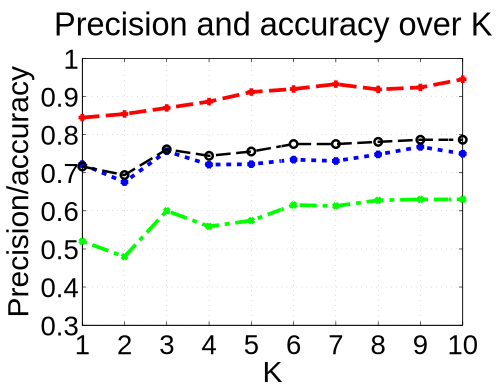
\includegraphics[width=0.3\textwidth]{tex/appendices/test/zcr11_P.png}
			\centering\includegraphics[width=0.3\textwidth]{tex/appendices/test/zcr11_R.png}
			\label{fig:eval:zcr}
			\caption{Plots over K for Zero Crossing Rate}
		\end{figure}
		
		\begin{table}
			\centering
			\begin{tabular}{|c|c|c|c"c|}
				\cline{2-5}
				 \multicolumn{1}{c|}{} & \textbf{k}  & \textbf{s}  & \textbf{hh}  & Prec.\\ \hline
				 \textbf{s} & \textcolor{red}{0.871} & 0.081 & 0.017 & 0.924\\ \hline
				 \textbf{k} & 0.122 & \textcolor{red}{0.636} & 0.169 & 0.630\\ \hline
				 \textbf{hh} & 0.122 & 0.283 & \textcolor{red}{0.814} & 0.768\\ \Xhline{2\arrayrulewidth}
				 F & 0.896 & 0.633 & 0.790 & \textcolor{blue}{0.787}\\ \hline
			\end{tabular}
			\label{table:eval:zcrBest1}
			\caption{$K=9$}
		\end{table}
		
		\begin{table}
			\centering
			\begin{tabular}{|c|c|c|c"c|}
				\cline{2-5}
				 \multicolumn{1}{c|}{} & \textbf{k}  & \textbf{s}  & \textbf{hh}  & Prec.\\ \hline
				 \textbf{s} & \textcolor{red}{0.871} & 0.051 & 0.017 & 0.945\\ \hline
				 \textbf{k} & 0.122 & \textcolor{red}{0.636} & 0.169 & 0.630\\ \hline
				 \textbf{hh} & 0.122 & 0.313 & \textcolor{red}{0.814} & 0.750\\ \Xhline{2\arrayrulewidth}
				 F & 0.906 & 0.633 & 0.780 & \textcolor{blue}{0.787}\\ \hline
			\end{tabular}
			\label{table:eval:zcrBest2}
			\caption{$K=10$}
		\end{table}
		
		\begin{table}
			\centering
			\begin{tabular}{|c|c|c|c"c|}
				\cline{2-5}
				 \multicolumn{1}{c|}{} & \textbf{k}  & \textbf{s}  & \textbf{hh}  & Prec.\\ \hline
				 \textbf{s} & \textcolor{red}{0.899} & 0.172 & 0.051 & 0.845\\ \hline
				 \textbf{k} & 0.101 & \textcolor{red}{0.525} & 0.288 & 0.520\\ \hline
				 \textbf{hh} & 0.101 & 0.303 & \textcolor{red}{0.661} & 0.722\\ \Xhline{2\arrayrulewidth}
				 F & 0.871 & 0.523 & 0.690 & \textcolor{blue}{0.716}\\ \hline
			\end{tabular}
			\label{table:eval:zcrWorst}
			\caption{$K=1$}
		\end{table}
		
		The best results using ZCR was a tie $K=9$ (table \ref{table:eval:zcrBest1) and $k=10$ (\ref{table:eval:zcrBest2}). In the results from $K=9$, the precision of the 'hh' is slightly better than in $K=10$. In $K=10$, the precision of the 'k' is slightly better.
		Th worst results was observed with $K=2$ (table \ref{table:eval:zcrWorst}). As with our results using RMS, we found that all probabilities were significant.
		
	%	
	%	MFCC
	%	
		
	\subsection{Mel Frequency Cepstrum Coefficients}
		\begin{figure}
		
		
			\centering\includegraphics[width=0.3\textwidth]{tex/appendices/test/mfcc2010FP.png}
			\centering\includegraphics[width=0.3\textwidth]{tex/appendices/test/mfcc2010_P.png}
			\centering\includegraphics[width=0.3\textwidth]{tex/appendices/test/mfcc2010_R.png}
			
			\caption{Plots over K for MFCC with 20ms windows and 10ms window skips}
		\end{figure}
		\begin{figure}
		
		
			\centering\includegraphics[width=0.3\textwidth]{tex/appendices/test/mfcc105FP.png}
			\centering\includegraphics[width=0.3\textwidth]{tex/appendices/test/mfcc105_P.png}
			\centering\includegraphics[width=0.3\textwidth]{tex/appendices/test/mfcc105_R.png}
			
			\caption{Plots over K for MFCC with 10ms windows and 5ms window skips}
		\end{figure}
		\begin{figure}
		
		
			\centering\includegraphics[width=0.3\textwidth]{tex/appendices/test/mfcc52FP.png}
			\centering\includegraphics[width=0.3\textwidth]{tex/appendices/test/mfcc52_P.png}
			\centering\includegraphics[width=0.3\textwidth]{tex/appendices/test/mfcc52_R.png}
			
			\caption{Plots over K for MFCC with 5ms windows and 2ms window skips}
		\end{figure}\clearpage
		
		% BEST:
		% WORST:
		
		
		
	\subsection{Spectral Centroid}
		\begin{figure}
		
		
			\centering\includegraphics[width=0.3\textwidth]{tex/appendices/test/scentroid2010FP.png}
			\centering\includegraphics[width=0.3\textwidth]{tex/appendices/test/scentroid2010_P.png}
			\centering\includegraphics[width=0.3\textwidth]{tex/appendices/test/scentroid2010_R.png}
			
			\caption{Plots over K for Spectral Centroid with 20ms windows and 10ms window skips}
		\end{figure}
		\begin{figure}
		
		
			\centering\includegraphics[width=0.3\textwidth]{tex/appendices/test/scentroid105FP.png}
			\centering\includegraphics[width=0.3\textwidth]{tex/appendices/test/scentroid105_P.png}
			\centering\includegraphics[width=0.3\textwidth]{tex/appendices/test/scentroid105_R.png}
				
				\caption{Plots over K for Spectral Centroid with 10ms windows and 5ms window skips}
		\end{figure}
		\begin{figure}
		
		
			\centering\includegraphics[width=0.3\textwidth]{tex/appendices/test/scentroid52FP.png}
			\centering\includegraphics[width=0.3\textwidth]{tex/appendices/test/scentroid52_P.png}
			\centering\includegraphics[width=0.3\textwidth]{tex/appendices/test/scentroid52_R.png}
				
				\caption{Plots over K for Spectral Centroid with 5ms windows and 2ms window skips}
		\end{figure}\clearpage
		
	
	
	\subsection{Spectral Skew}
			
		\begin{figure}
		
		
			\centering\includegraphics[width=0.3\textwidth]{tex/appendices/test/sskew2010FP.png}
			\centering\includegraphics[width=0.3\textwidth]{tex/appendices/test/sskew2010_P.png}
			\centering\includegraphics[width=0.3\textwidth]{tex/appendices/test/sskew2010_R.png}
			
			\caption{Plots over K for Spectral Skew with 20ms windows and 10ms window skips}
		\end{figure}
		
		\begin{figure}
		
		
			\centering\includegraphics[width=0.3\textwidth]{tex/appendices/test/sskew105FP.png}
			\centering\includegraphics[width=0.3\textwidth]{tex/appendices/test/sskew105_P.png}
			\centering\includegraphics[width=0.3\textwidth]{tex/appendices/test/sskew105_R.png}
				
				\caption{Plots over K for Spectral Skew with 10ms windows and 5ms window skips}
		\end{figure}
		\begin{figure}
		
		
			\centering\includegraphics[width=0.3\textwidth]{tex/appendices/test/sskew52FP.png}
			\centering\includegraphics[width=0.3\textwidth]{tex/appendices/test/sskew52_P.png}
			\centering\includegraphics[width=0.3\textwidth]{tex/appendices/test/sskew52_R.png}
				
				\caption{Plots over K for Spectral Skew with 5ms windows and 2ms window skips}
		\end{figure}\clearpage
		
	
	
	\subsection{Spectral Flux}
		
		\begin{figure}
		
		
			\centering\includegraphics[width=0.3\textwidth]{tex/appendices/test/sflux2010FP.png}
			\centering\includegraphics[width=0.3\textwidth]{tex/appendices/test/sflux2010_P.png}
			\centering\includegraphics[width=0.3\textwidth]{tex/appendices/test/sflux2010_R.png}
			
			\caption{Plots over K for Spectral Flux with 20ms windows and 10ms window skips}
		\end{figure}
		\begin{figure}
		
		
			\centering\includegraphics[width=0.3\textwidth]{tex/appendices/test/sflux105FP.png}
			\centering\includegraphics[width=0.3\textwidth]{tex/appendices/test/sflux105_P.png}
			\centering\includegraphics[width=0.3\textwidth]{tex/appendices/test/sflux105_R.png}
				
				\caption{Plots over K for Spectral Flux with 10ms windows and 5ms window skips}
		\end{figure}
		\begin{figure}
		
		
			\centering\includegraphics[width=0.3\textwidth]{tex/appendices/test/sflux52FP.png}
			\centering\includegraphics[width=0.3\textwidth]{tex/appendices/test/sflux52_P.png}
			\centering\includegraphics[width=0.3\textwidth]{tex/appendices/test/sflux52_R.png}
				
				\caption{Plots over K for Spectral Flux with 5ms windows and 2ms window skips}
		\end{figure}
		



\chapter{Discussion}
\thispagestyle{empty}

\chapter{Conclusion}
\thispagestyle{empty}

\bibliography{sources}
\bibliographystyle{apalike}

\begin{appendices}
\chapter{Matlab Scripts}
\section{Features}
\label{app:features}
% SPECTROGRAM ---- START
\subsection{Spectrogram}
\label{app:feat-spectrogram}

\begin{lstlisting}[caption=Matlab implementation of calculating the spectrogram., label=snippet-spectrogram]
function spec = P4_Spectrogram(signal, fs, winSize, winSkip)
    % spec = P4_Spectrogram(signal, fs, winSize, winSkip)
    % Calculates the mean spectral centroid of a signal
    %
    % @param signal:    signal vector
    % @param fs:        sampling rate of signal X
    % @param winSize:   analysis window size in seconds
    % @param winSkip:   amount to shift each window in seconds
    
    % Make it a column vector
    if isrow(signal)
        signal = signal';
    end
    
    win_size = winSize * fs;
    win_skip = winSkip * fs;
    wins = 1 + floor((length(signal)-win_size)/win_skip);
    
    L       = win_size;             % Length of each window
    NFFT    = 2^nextpow2(L);        % Length of the fft
    spec    = zeros(NFFT/2+1, wins);% Allocating mem. to spectrogram
    
    for ii = 1:wins
        start = floor((ii-1) * win_skip) + 1;
        stop = floor((ii-1) * win_skip + win_size);
        window = signal(start:stop,1);
        
        Y = fft(window,NFFT)/L;
        spec(:,ii) = 2*abs(Y(1:NFFT/2+1));
    end
end
\end{lstlisting}
% SPECTROGRAM ---- END

% CENTROID ---- START
\subsection{Spectral Centroid}
\label{app:feat-centroid}

\begin{lstlisting}[caption=Matlab implementation of the spectral centroid., label=snippet-speccentroid] 
function [sct] = P4_MeanSpectralCentroid(signal, fs, winSize, winSkip)
    % sct = P4_SpectralCentroid(X, fs)
    % Calculates the mean spectral centroid of a signal
    %
    % @param X:         signal vector
    % @param fs:        sampling rate of signal X
    % @param winSize:   analysis window size in seconds
    % @param winSkip:   amount to shift each window in seconds
    
    spec = P4_Spectrogram(signal, fs, winSize, winSkip);
    sct = mean(SpectralCentroid(spec, fs));
end

function vsc = SpectralCentroid(X, fs)
% Credit: Alexander Lerch, An Introduction to Audio Content Analysis.
% ===================================================================
% @brief computes the spectral centroid from the (squared) magnitude spectrum
%
% @param X: spectrogram (dimension FFTLength X Observations)
% @param f_s: sample rate of audio data 
%
% @retval v spectral centroid (in Hz)
    X       = X.^2;
    vsc     = ([0:size(X,1)-1]*X)./sum(X,1);
 
    % avoid NaN for silence frames
    vsc (sum(X,1) == 0) = 0;
 
    % convert from index to Hz
    vsc     = vsc / size(X,1) * fs/2;
end
\end{lstlisting}
% CENTROID ---- END

% FLUX ---- START
\subsection{Spectral Flux}
\label{app:feat-flux}

\begin{lstlisting}[caption=Matlab implementation of the spectral flux., label=snippet-specflux]
function [sflx] = P4_MeanSpectralFlux(signal, fs, winSize, winSkip)
    % sct = P4_SpectralCentroid(X, fs)
    % Calculates the mean spectral centroid of a signal
    %
    % @param X:         signal vector
    % @param fs:        sampling rate of signal X
    % @param winSize:   analysis window size in seconds
    % @param winSkip:   amount to shift each window in seconds
    
   spec = P4_Spectrogram(signal, fs, winSize, winSkip);
   sflx = mean(SpectralFlux(spec));
end

function [vsf] = SpectralFlux (X)
% Credit: Alexander Lerch, An Introduction to Audio Content Analysis.
% ===================================================================
% @brief computes the spectral flux from the magnitude spectrum
% called by ::ComputeFeature
%
% @param X: spectrogram (dimension FFTLength X Observations)
%
% @retval v spectral flux

    % difference spectrum (set first diff to zero)
    afDeltaX    = diff([X(:,1), X],1,2);
 
    % flux
    vsf         = sqrt(sum(afDeltaX.^2))/size(X,1);
end
\end{lstlisting}
% FLUX ---- END

% ROLLOFF ---- START
\subsection{Spectral Rolloff}
\label{app:feat-rolloff}

\begin{lstlisting}[caption=Matlab implementation of the spectral rolloff., label=snippet-specrolloff]
function sroff = P4_MeanSpectralRolloff(signal, fs, winSize, winSkip)
    spec = P4_Spectrogram(signal, fs, winSize, winSkip);
    sroff = mean(SpectralRolloff(spec, fs));
end

function [vsr] = SpectralRolloff (X, fs, kappa)
% Credit: Alexander Lerch, An Introduction to Audio Content Analysis.
% ===================================================================
% @brief computes the spectral rolloff from the magnitude spectrum
%
% @param X: spectrogram (dimension FFTLength X Observations)
% @param fs: sample rate of audio data 
%
% @retval v spectral rolloff (in Hz)

    % initialize parameters
    if (nargin < 3)
        kappa   = 0.85;
    end
 
    % allocate memory
    vsr     = zeros(1,size(X,2));
 
    %compute rolloff
    afSum   = sum(X,1);
    for (n = 1:length(vsr))
        vsr(n)  = find(cumsum(X(:,n)) >= kappa*afSum(n), 1); 
    end
 
    % convert from index to Hz
    vsr     = vsr / size(X,1) * fs/2;
end
\end{lstlisting}
% ROLLOFF ---- END

% SKEWNESS ---- START
\subsection{Spectral Skewness}
\label{app:feat-skewness}

\begin{lstlisting}[caption=Matlab implementation of the spectral skewness., label=snippet-specskewness]
function sskw = P4_MeanSpectralSkewness(signal, fs, winSize, winSkip)
    % sskw = P4_SpectralSkewness(X, fs)
    % Calculates the spectral skewness of a signal
    %
    % @param X:         signal vector
    % @param fs:        sampling rate of signal X
    % @param winSize:   analysis window size in seconds
    % @param winSkip:   amount to shift each window in seconds
    
    spec = P4_Spectrogram(signal, fs, winSize, winSkip);
    sskw = mean(SpectralSkewness(spec));
end

function [vssk] = SpectralSkewness (X)
% Credit: Alexander Lerch, An Introduction to Audio Content Analysis.
% ===================================================================
% @brief computes the spectral skewness from the magnitude spectrum
% called by ::ComputeFeature
%
% @param X: spectrogram (dimension FFTLength X Observations)
%
% @retval v spectral skewness
    UseBookDefinition = true;
 
    if (UseBookDefinition)
        % compute mean and standard deviation
        mu_x    = mean(abs(X), 1);
        std_x   = std(abs(X), 1);
 
        % compute skewness
        X       = X - repmat(mu_x, size(X,1), 1);
        vssk    = sum ((X.^3)./(repmat(std_x, size(X,1), 1).^3*size(X,1)));
    else
        % interpret the spectrum as pdf, not as signal
        f       = linspace(0, fs/2, size(X,1));
        % compute mean and standard deviation
        mu_X    = (f * X) ./ (sum(X,1));
        tmp     = repmat(f, size(X,2),1) - repmat(mu_X, size(X,1),1)';
        var_X   = diag (tmp.^2 * X) ./ (sum(X,1)'*size(X,1));
 
        vssk    = diag (tmp.^3 * X) ./ (var_X.^(3/2) .* sum(X,1)'*size(X,1));
    end
 
    % avoid NaN for silence frames
    vssk (sum(X,1) == 0) = 0;
end
\end{lstlisting}
% SKEWNESS ---- END

\end{appendices}
\end{document}